%%%%%%%%%%%%%%%%%%%%%%%%%%%%%%%%%%%%%%%%%%%%%%%%%%%%%%%%%%%%%%%%%%%%%%%%%%%%%%%
\section{Test Cases and Reference Results}
\label{sec:test-cases}
%%%%%%%%%%%%%%%%%%%%%%%%%%%%%%%%%%%%%%%%%%%%%%%%%%%%%%%%%%%%%%%%%%%%%%%%%%%%%%%

This paper models two test cases derived from the Benchmark for Evaluation And Validation of Reactor Simulations (BEAVRS) PWR model~\citep{horelik2013beavrs}. Each test case includes heterogeneous features -- and corresponding spatial self-shielding effects -- in order to understand their implications for accurate pin-wise MGXS generation. Although BEAVRS is an axially heterogeneous 3D core model, both benchmarks were fabricated in 2D due to the geometric constraints in OpenMOC. The impact of fuel enrichment, CRGTs, BPs, inter-assembly currents and water reflectors is considered. The geometric and material specifications for the two test cases are summarized in~\autoref{subsec:benchmarks}. The reference results computed with OpenMC are discussed in~\autoref{subsec:metrics}.


%%%%%%%%%%%%%%%%%%%%%%%%%%%%%%%%%%%%%%%%%%%%%%%%%%%%%%%%%%%%%%%%%%%%%%%%%%%%%%%
\subsection{Benchmark Configurations}
\label{subsec:benchmarks}

The two test cases were comprised of materials from the BEAVRS model, including 1.6\% and 3.1\% enriched UO$_2$ fuel, borated water\footnote{The water consisted of 975 parts per million (ppm) boron.}, zircaloy, helium, air, borosilicate glass and stainless steel. The densities and isotopic compositions for each material are detailed in the BEAVRS specifications~\citep{horelik2013beavrs}. Each material was modeled with cross sections from the ENDF/B-VII.1 continuous energy cross section library~\citep{mcnpx2003manual} evaluated at 600K for hot zero power conditions.

The first benchmark was a single fuel assembly with an array of 264 fuel pins of 1.6\% enriched UO$_2$ fuel with zircaloy cladding and a helium gap as illustrated in~\autoref{fig:benchmarks-assm}. The assembly included 24 CRGTs of borated water surrounded by zircaloy cladding, and a central instrument tube filled with air surrounded by two zircaloy tubes separated by borated water. The intra-pin egg-crate grid spacer and grid sleeve separating each assembly in the BEAVRS model were not included in the assembly benchmark. The assembly was modeled with reflective boundary conditions.

The second benchmark was constructed as a 2$\times$2 colorset of two fuel assemblies extracted from the BEAVRS model. The top-left and bottom-right fuel assemblies in the colorset were of the same enrichment and configuration as the first benchmark configuration. The top-right and bottom-left fuel assemblies included 264 fuel pins of 3.1\% enriched UO$_2$ fuel, 20 CRGTs and a central instrument tube. In addition, the two 3.1\% enriched assemblies included four BPs consisting of eight layers of air, steel, borosilicate glass and zircaloy. The colorset was surrounded by a water reflector on the bottom and right that was of the same width as a fuel assembly. The reflected colorset included reflective boundaries on the top and left (adjacent to the fuel assemblies) with vacuum boundaries on the bottom and right (adjacent to the reflector).

%The colorset does not include the stainless steel baffle surrounding the fuel assemblies adjacent to the water reflector in the full core BEAVRS model.

\begin{figure}[ht!]
\centering
\begin{subfigure}{0.45\textwidth}
  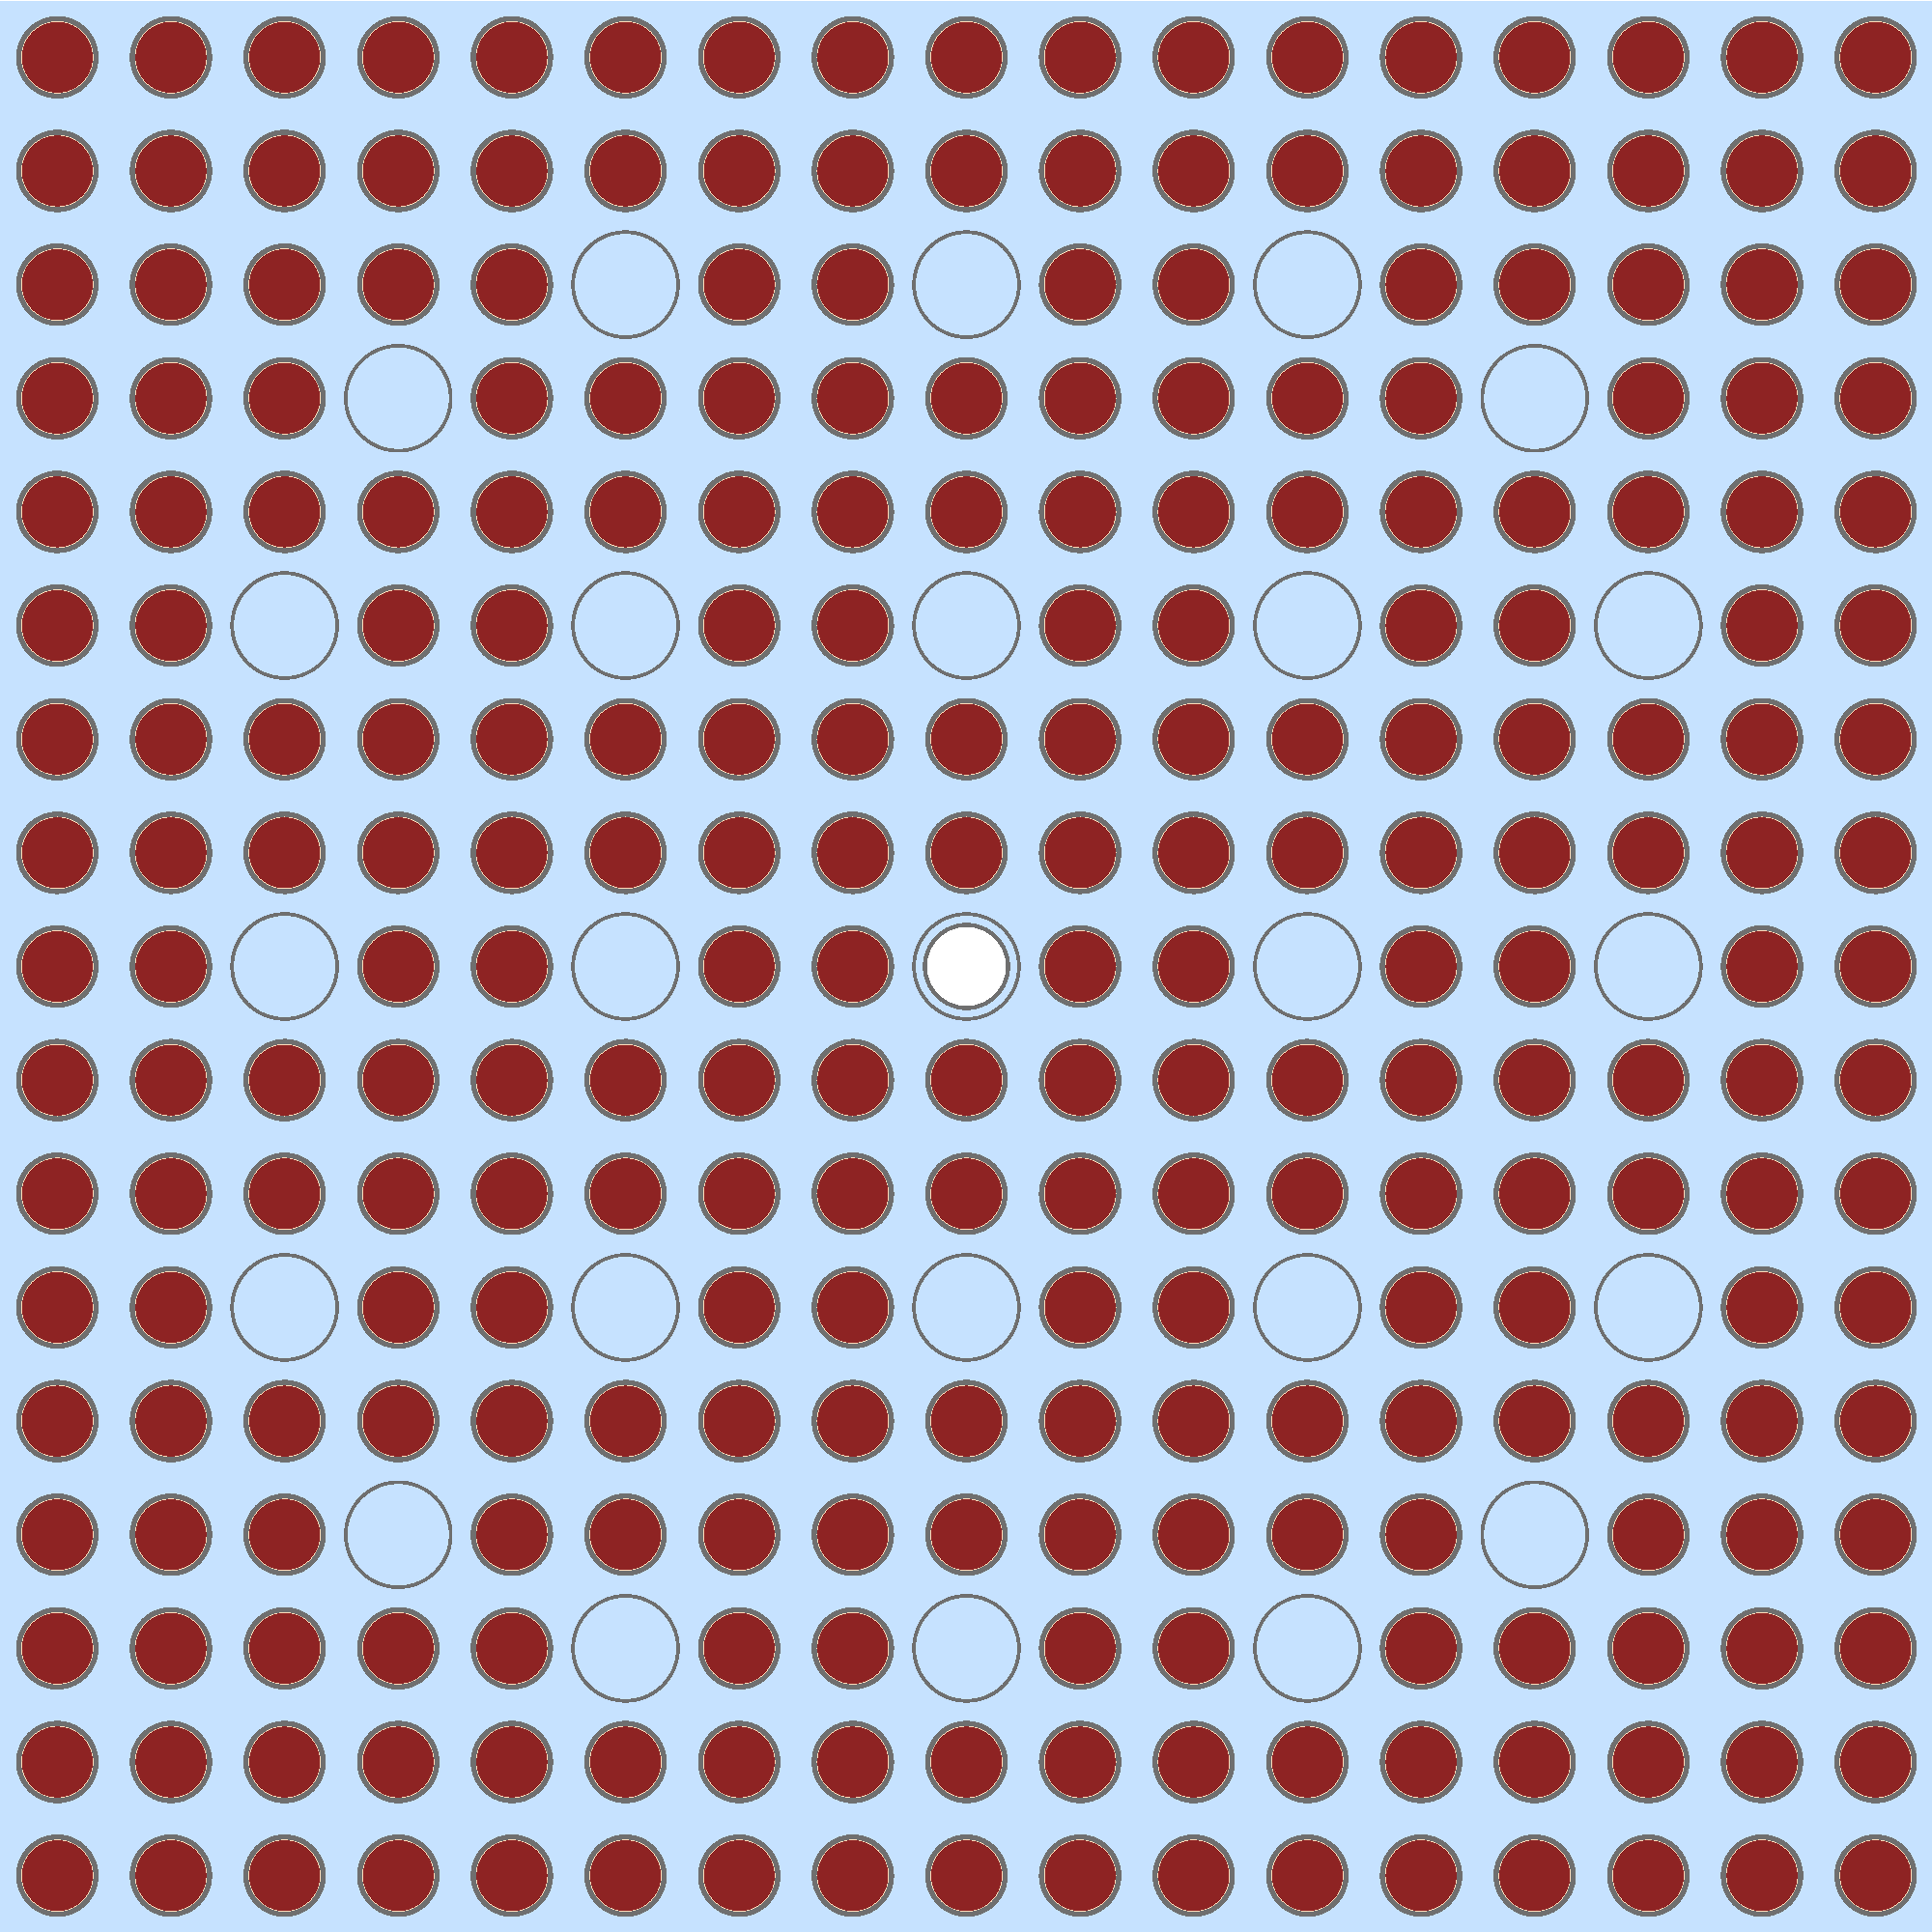
\includegraphics[width=\linewidth]{figures/assembly/geometry}
  \caption{}
  \label{fig:benchmarks-assm}
\end{subfigure}
\begin{subfigure}{0.45\textwidth}
  \centering
  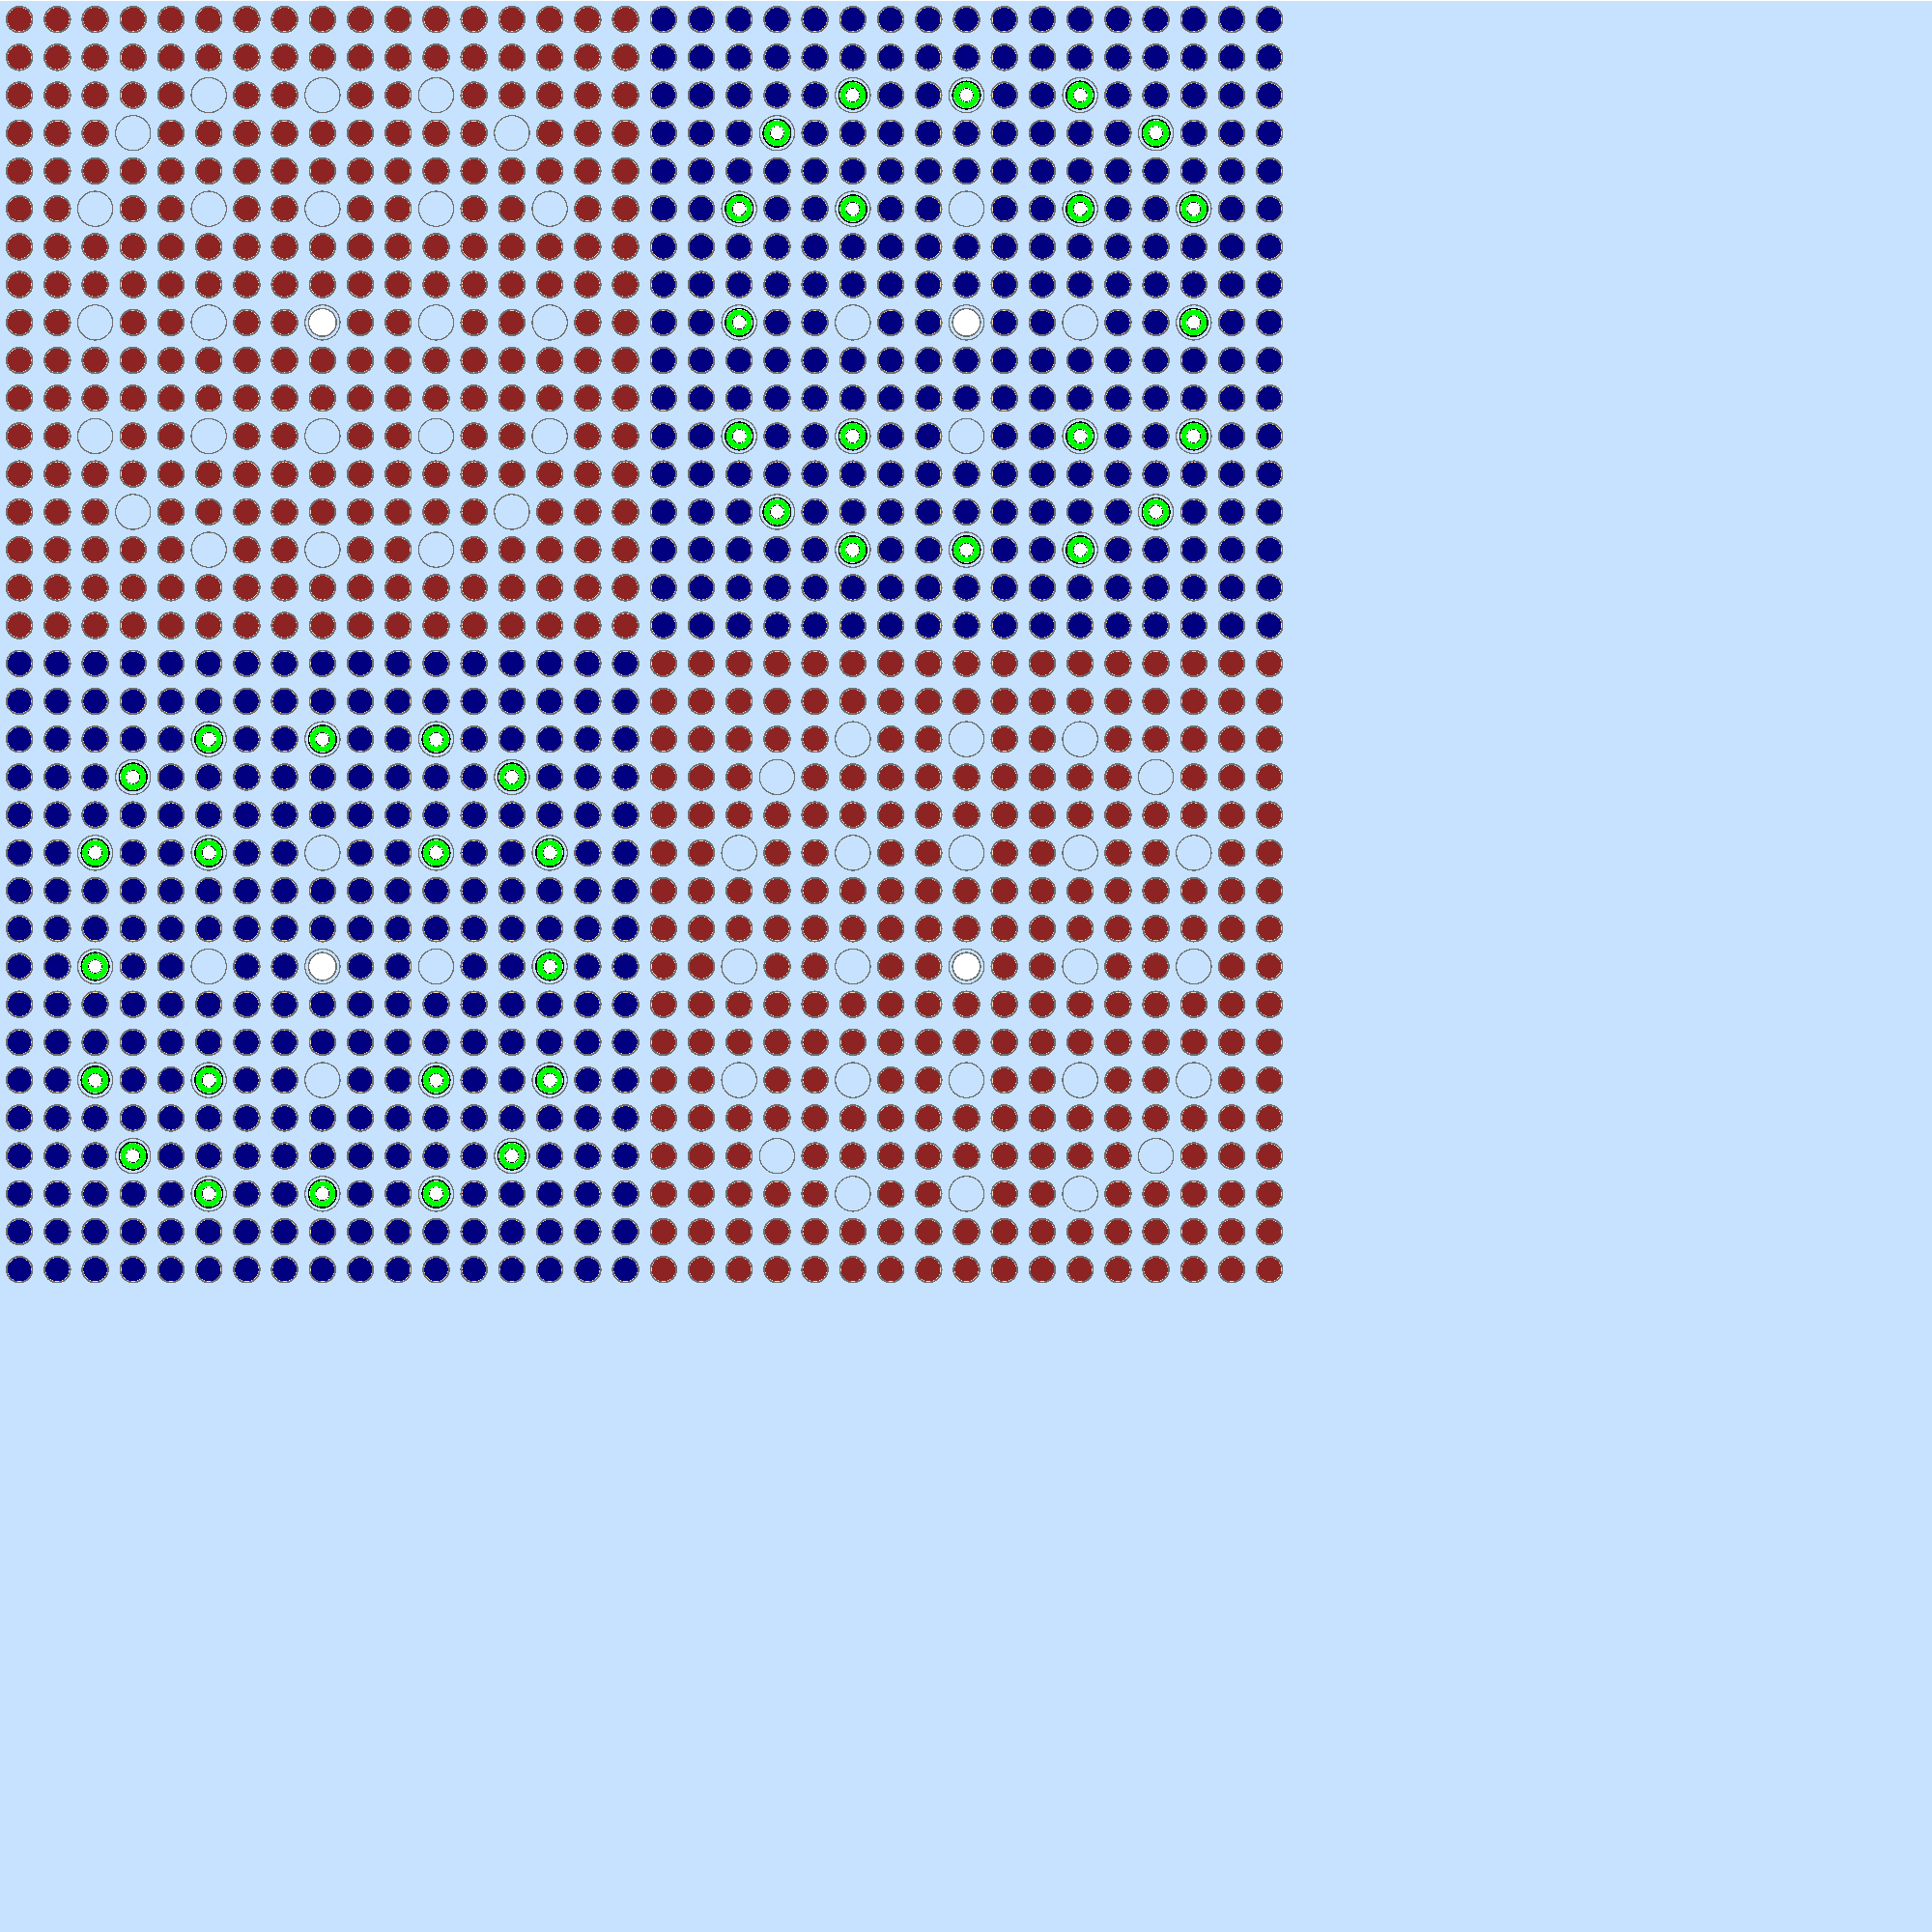
\includegraphics[width=\linewidth]{figures/reflector/geometry}
  \caption{}
  \label{fig:benchmarks-reflector}
\end{subfigure}
\caption{A (a) fuel assembly and (b) 2$\times$2 assembly colorset with reflector.}
\label{fig:benchmarks}
\end{figure}


%%%%%%%%%%%%%%%%%%%%%%%%%%%%%%%%%%%%%%%%%%%%%%%%%%%%%%%%%%%%%%%%%%%%%%%%%%%%%%%
\subsection{Verification Metrics}
\label{subsec:metrics}

A series of OpenMC simulations were used to calculate reference eigenvalues, pin-wise fission rates, and pin-wise U-238 capture rates for both benchmarks. The reference solutions were computed with 100 inactive and 900 active batches of 10$^7$ particle histories per batch. The reference eigenvalues are listed in~\autoref{tab:keff-reference}. The OpenMC ``combined'' eigenvalue estimator is reported along with the associated 1-sigma uncertainty of one pcm for both test cases.

%It should be noted that isotropic in lab scattering was employed for all reference calculations with OpenMC's ``iso-in-lab'' feature\footnote{The OpenMC ``iso-in-lab'' feature samples the outgoing neutron energy from the scattering laws prescribed by the continuous energy cross section library, but the outgoing neutron direction of motion is sampled from an isotropic in lab distribution.}. Although isotropic in lab scattering is a poor approximation for LWRs, it eliminated scattering source anisotropy as one possible cause of approximation error between OpenMC and OpenMOC in order to isolate approximation errors resulting from spatially self-shielded MGXS.

\begin{table}[h!]
  \centering
  \caption{Reference OpenMC eigenvalues for each test case.}
  \label{tab:keff-reference} 
  \begin{tabular}{c c}
  \toprule
  {\bf Assembly} &
  {\bf Colorset} \\
  \midrule
  0.99326 $\pm$ 0.00001 & 0.94574 $\pm$ 0.00001 \\
  \bottomrule
\end{tabular}
\end{table}

The reference energy-integrated fission and U-238 capture rate spatial distributions were computed using rectilinear, pin-wise tally meshes in OpenMC and are shown in~\autoref{fig:fiss-capt-rates}. The reaction rates were volume-integrated across each fuel pin. The fission rates include fission from only U-235 and U-238 for the fresh PWR UO$_2$ fuel. The reaction rates were normalized to the mean of all non-zero reaction rates in each benchmark. The reaction rates in the instrument tubes, CRGTs and BPs are all zero and are illustrated in white. The 1-sigma uncertainties are less than 0.08\% in each pin for each benchmark.

\begin{figure*}[h!]
\centering
\begin{subfigure}{0.45\textwidth}
  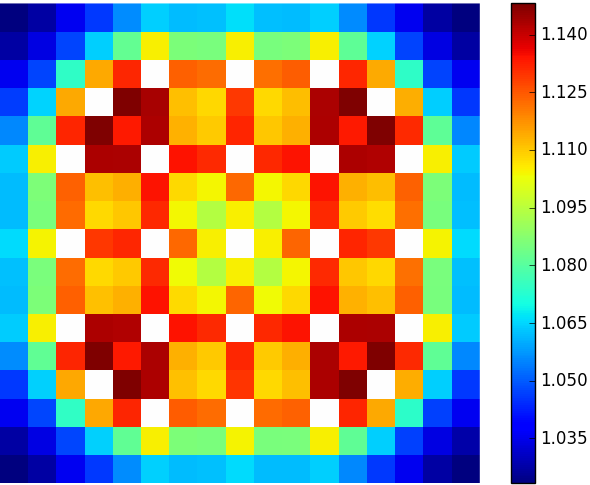
\includegraphics[width=\linewidth]{figures/assembly/fission-rates}
  \caption{}
  \label{fig:fiss-assm}
\end{subfigure}%
\begin{subfigure}{0.45\textwidth}
  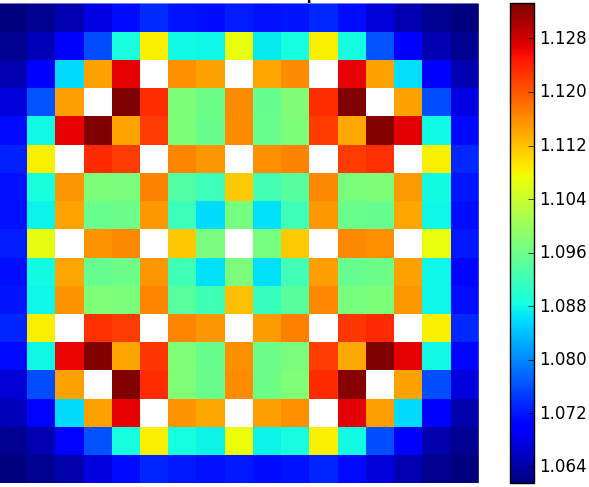
\includegraphics[width=\linewidth]{figures/assembly/capture-rates}
  \caption{}
  \label{fig:capt-assm}
\end{subfigure}
\begin{subfigure}{0.45\textwidth}
  \centering
  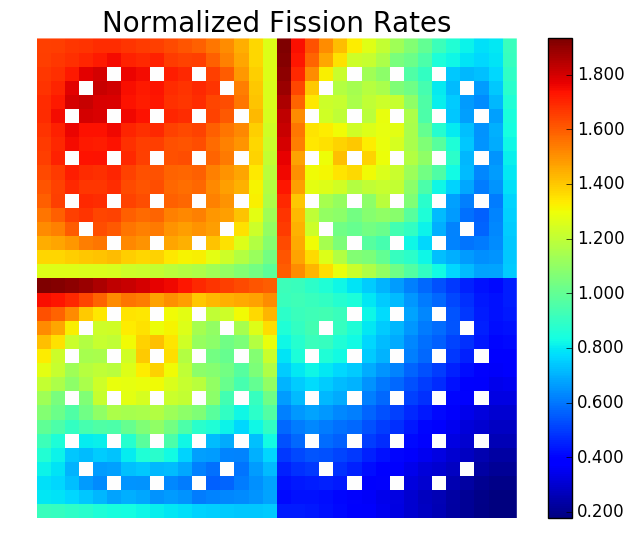
\includegraphics[width=\linewidth]{figures/reflector/fission-rates}
  \caption{}
  \label{fig:fiss-reflector}
\end{subfigure}%
\begin{subfigure}{0.45\textwidth}
  \centering
  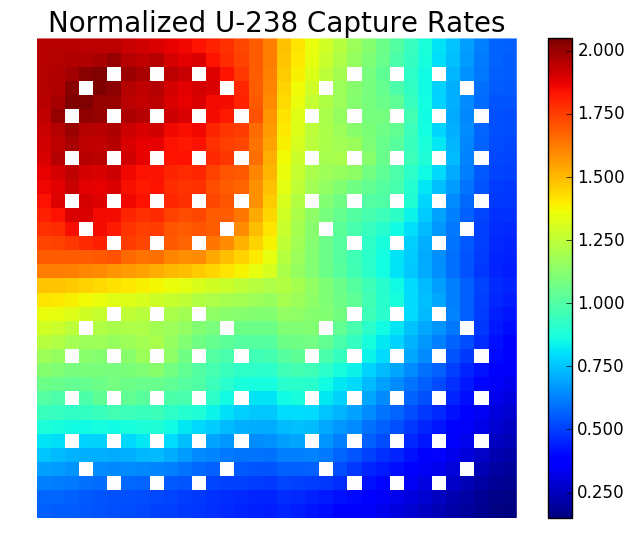
\includegraphics[width=\linewidth]{figures/reflector/capture-rates}
  \caption{}
  \label{fig:capt-reflector}
\end{subfigure}
\caption{Fission and U-238 capture rates for the (a) -- (b) assembly and (c) -- (d) colorset.}
\label{fig:fiss-capt-rates}
\end{figure*}

As illustrated in the figures, the reaction rate rate distributions are strongly dependent on the spatially heterogeneous features in each benchmark. For example, the CRGTs provide additional moderation and increase the fision and U-238 capture rates in nearby fuel pins. The inclusion of BPs reduces the neutron population and therefore the reaction rates for the surrounding fuel pins. The presence of a reflector with a mixture of vacuum and reflective BCs induces a tilt in the reaction rates across the assemblies in the colorset.

Although spatial heterogeneities generally have similar effects on both fission and U-238 capture rates, there are a few important differences to note. The U-238 capture rates in the assemblies are more sensitive than the fission rates to the spatial self-shielding induced by moderation in CRGTs. In addition, the capture rates in the colorset are more smoothly varying at the inter-assembly and assembly-reflector interfacea than the fission rates.